\documentclass{book}

\usepackage[total={20cm,21cm},top=2cm, left=2cm]{geometry}
\usepackage{amsmath,amssymb,amsfonts,latexsym,stmaryrd}
\usepackage{tikz}
%--

\begin{document}

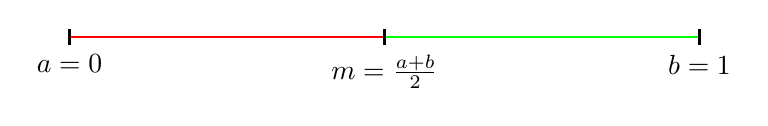
\begin{tikzpicture}[xscale=8]
  % Segmento de 0 a 1
\draw[-][draw=red,   thick] (0,0) -- (.5,0);
\draw[-][draw=green, thick] (.5,0) -- (1,0);
  % Texto debajo ("below") del segmento
\draw [thick] (0,-.1)    node[below]{$a=0$}             -- (0,0.1);
\draw [thick] (0.5,-.1) node[below]{$m=\frac{a+b}{2}$} -- (0.5,0.1);
\draw [thick] (1,-.1)    node[below]{$b=1$}             -- (1,0.1);
\end{tikzpicture}

\end{document}